\documentclass[twocolumn,9pt]{extarticle}
\usepackage[a4paper,margin=1.7cm,top=1.8cm,bottom=1.8cm,heightrounded]{geometry}
\usepackage[T1]{fontenc}
\usepackage[utf8]{inputenc}

\usepackage{microtype}
\usepackage{amsmath,amsthm}
\usepackage{newtxtext,newtxmath}
\usepackage[varqu,varl,scaled=0.96]{inconsolata}   %
\usepackage{booktabs,array,float}
\usepackage{graphicx}
\usepackage{xcolor}
\usepackage{tikz}
\usetikzlibrary{arrows.meta,positioning,calc}

\definecolor{ink}{RGB}{28,31,36}          %
\definecolor{accent}{RGB}{38,66,98}       %
\definecolor{link}{RGB}{52,92,136}        %
\definecolor{note}{RGB}{110,116,126}      %
\definecolor{rulegray}{RGB}{160,165,172}  %
\definecolor{todo}{RGB}{178,40,40}        %
\definecolor{pholder}{RGB}{176,104,0}     %
\color{ink}

\usepackage[ruled,linesnumbered,noend]{algorithm2e}
\usepackage{etoolbox}
\DontPrintSemicolon
\SetAlgoLined
\SetAlFnt{\footnotesize\lineskiplimit=0pt\lineskip=1pt}
\SetAlCapFnt{\small\bfseries}\SetAlCapNameFnt{\small}
\SetAlgoCaptionSeparator{.}
\SetAlgoNlRelativeSize{-1}
\newcommand{\algnl}[1]{\textcolor{note}{#1}}
\SetNlSty{algnl}{}{}
\newcommand{\algcmt}[1]{\textcolor{note}{\itshape #1}}
\SetCommentSty{algcmt}
\SetKwComment{tcp}{$\triangleright$\ }{}
\newcommand{\algkw}[1]{\textcolor{accent}{\textbf{#1}}}
\SetKwSty{algkw}
\SetArgSty{textnormal}
\renewcommand{\ProgSty}[1]{\textnormal{#1}\unskip}%
\newcommand{\AlgFn}[2]{\textsc{#1}\textnormal{(#2)}}
\SetInd{0.45em}{0.85em}
\setlength{\algomargin}{1.3em}
\SetAlgoSkip{}
\SetAlgoInsideSkip{}
\setlength{\interspacetitleruled}{3pt}
\setlength{\interspacealgoruled}{3pt}
\makeatletter
\AtBeginDocument{\setlength{\algoheightrule}{\heavyrulewidth}\setlength{\algotitleheightrule}{\lightrulewidth}}
\def\@algocf@pre@ruled{{\color{accent}\hrule width\algocf@ruledwidth height\algoheightrule depth0pt}\kern\interspacetitleruled}
\def\@algocf@post@ruled{\kern\interspacealgoruled{\color{accent}\hrule width\algocf@ruledwidth height\algoheightrule}\relax}
\renewcommand{\algocf@caption@ruled}{\box\algocf@capbox\kern\interspacetitleruled
  {\color{accent}\hrule width\algocf@ruledwidth height\algotitleheightrule depth0pt}\kern\interspacealgoruled}
\renewcommand{\algocf@Vsline}[1]{%
  \strut\par\nointerlineskip
  \algocf@bblockcode
  \algocf@push{\skiprule}%
  \hbox{{\color{rulegray}\vrule width 0.3pt}%
    \vtop{\algocf@push{\skiptext}%
      \vtop{\algocf@addskiptotal #1}}}%
  \algocf@pop{\skiprule}%
  \algocf@eblockcode}
\newlength{\alglabelw}\newlength{\algsymw}
\newcommand{\alg@newrow}{\par\noindent\hskip\alglabelw\ignorespaces}
\newcommand{\alg@head}[2]{%
  \settowidth{\alglabelw}{\algkw{Constants}\enspace}%
  \algocf@seteveryparnl{\relax}%
  {\let\\\alg@newrow\rightskip=0pt plus 2em\relax
   \noindent\hbox to\alglabelw{\algkw{#1}\hfil}#2\par}%
  \algocf@linesnumbered}
\newcommand{\AlgIn}[1]{\alg@head{Input}{#1}}
\newcommand{\AlgOut}[1]{\alg@head{Output}{#1}}
\newcommand{\AlgNote}[1]{\alg@head{Notation}{#1}}
\newcommand{\AlgConst}[1]{\alg@head{Constants}{#1}}
\setlength{\algsymw}{2.7em}
\newcommand{\AlgRow}[2]{\hangindent=\dimexpr\alglabelw+\algsymw\relax\hangafter=1\relax
  \makebox[\algsymw][l]{#1}#2}
\newcommand{\AlgWide}[1]{\hangindent=\alglabelw\hangafter=1\relax #1}
\newcommand{\AlgBody}{\par\nointerlineskip\vskip 2.5pt
  \moveleft\algomargin\vbox{\color{rulegray}\hrule width\algocf@ruledwidth height 0.3pt}%
  \vskip 2.5pt}
\makeatother

\usepackage[round,authoryear,sort]{natbib}
\usepackage{url}
\usepackage[colorlinks=true,linkcolor=link,citecolor=link,urlcolor=link]{hyperref}
\usepackage{caption}
\captionsetup{font=small,labelfont=bf,labelsep=period,skip=5pt}
\usepackage{titlesec}
\titleformat{\section}{\large\bfseries}{\textcolor{accent}{\thesection}}{0.6em}{\color{accent}}
\titleformat{\subsection}{\normalsize\bfseries}{\thesubsection}{0.6em}{}
\titleformat{\subsubsection}{\normalsize\itshape}{\thesubsubsection}{0.6em}{}
\setlength{\columnsep}{0.6cm}
\linespread{1.0}
\setlength{\parskip}{0pt}
\newcommand{\GridLinePitch}{\normallineskiplimit=-2.5pt \normallineskip=0pt
  \lineskiplimit=\normallineskiplimit \lineskip=\normallineskip}%
\titlespacing*{\section}{0pt}{9.9pt plus 4pt minus 1pt}{0pt}
\titlespacing*{\subsection}{0pt}{10.95pt plus 4pt minus 1pt}{0pt}
\titlespacing*{\subsubsection}{0pt}{10.95pt plus 4pt minus 1pt}{0pt}
\makeatletter
\g@addto@macro\normalsize{%
  \abovedisplayskip 5.475pt plus 1.5pt minus 1pt \belowdisplayskip\abovedisplayskip
  \abovedisplayshortskip\abovedisplayskip \belowdisplayshortskip\abovedisplayskip}
\makeatother
\normalsize
\setlength{\textfloatsep}{13pt plus 3pt minus 2pt}
\setlength{\floatsep}{13pt plus 3pt minus 2pt}
\setlength{\intextsep}{13pt plus 3pt minus 2pt}
\setlength{\dbltextfloatsep}{13pt plus 3pt minus 2pt}
\setlength{\dblfloatsep}{13pt plus 3pt minus 2pt}
\renewcommand{\topfraction}{0.9}\renewcommand{\bottomfraction}{0.8}\renewcommand{\textfraction}{0.1}
\renewcommand{\floatpagefraction}{0.85}\renewcommand{\dbltopfraction}{0.9}\renewcommand{\dblfloatpagefraction}{1}
\setcounter{topnumber}{3}\setcounter{bottomnumber}{2}\setcounter{totalnumber}{4}\setcounter{dbltopnumber}{1}%
\makeatletter
\newdimen\grid@bs \newdimen\grid@pad \newcount\grid@n
\AtBeginDocument{\grid@bs=\baselineskip}
\patchcmd\@cflb{\vskip \textfloatsep}{\vskip \textfloatsep \vskip \z@ \@plus 1fil\relax}{}{\PackageWarningNoLine{layout}{could not patch \string\@cflb}}
\let\grid@endfloatbox\@endfloatbox
\def\@endfloatbox{\grid@endfloatbox\grid@snapfloat}
\def\grid@snapfloat{%
  \@tempcnta=\count\@currbox \divide\@tempcnta 2 %
  \ifodd\@tempcnta
    \@tempdima=\dimexpr\ht\@currbox+\dp\@currbox+\textfloatsep\relax
    \grid@n=\numexpr(\@tempdima+\grid@bs/2-1)/\grid@bs\relax
    \grid@pad=\dimexpr\grid@n\grid@bs-\@tempdima\relax
    \ifdim\grid@pad>\z@
      \global\setbox\@currbox\vbox{\unvbox\@currbox\vskip\grid@pad}%
    \fi
  \fi}
\makeatother
\bibliographystyle{plainnat}

\newtheorem{proposition}{Proposition}
\newcommand{\flash}{FlashAlign}  %
\newcommand{\mmtwo}{minimap2}
\newcommand{\todo}[1]{\textcolor{todo}{[TODO: #1]}}
\newcommand{\placeholder}[1]{\textcolor{pholder}{\textbf{[PLACEHOLDER: #1]}}}

\renewenvironment{abstract}{%
  \par\noindent{\color{accent}\rule{\textwidth}{0.6pt}}\par\vspace{6pt}%
  \begin{list}{}{\setlength{\leftmargin}{0.5cm}\setlength{\rightmargin}{0.5cm}%
    \setlength{\topsep}{0pt}\setlength{\parsep}{0pt}\setlength{\itemsep}{0pt}\setlength{\listparindent}{0pt}}%
  \item\relax\normalsize}
 {\end{list}\par\vspace{6pt}\noindent{\color{rulegray}\rule{\textwidth}{0.4pt}}\par}

\title{\vspace{-1.2em}\LARGE\bfseries \flash: Faster Long-Read Alignment with Better Chaining\vspace{-0.3em}}
\author{Gong Chen$^{1,*}$ and Ian Korf$^{1,2,*}$\\[0.3em]
\small $^1$Genome Center, University of California, Davis, CA 95616, USA\\
\small $^2$Department of Molecular and Cellular Biology, University of California, Davis, CA 95616, USA\\
\small $^*$Corresponding authors: \texttt{dsbchen@ucdavis.edu}, \texttt{ifkorf@ucdavis.edu}}
\date{\small Preprint, \today}

\newcommand{\BodySpacing}{%
  \setlength{\parskip}{4.5pt plus 1.5pt minus 1pt}%
  \titlespacing*{\section}{0pt}{18pt plus 4pt minus 2pt}{3pt plus 1pt}%
  \titlespacing*{\subsection}{0pt}{13.5pt plus 3pt minus 1.5pt}{2pt plus 0.5pt}%
  \titlespacing*{\subsubsection}{0pt}{11pt plus 3pt minus 1pt}{1.5pt plus 0.5pt}%
  \raggedbottom
}
\AtBeginEnvironment{algorithm}{\setlength{\parskip}{0pt}}
\AtBeginEnvironment{figure}{\setlength{\parskip}{0pt}}
\AtBeginEnvironment{figure*}{\setlength{\parskip}{0pt}}
\AtBeginEnvironment{table}{\setlength{\parskip}{0pt}}
\AtBeginEnvironment{table*}{\setlength{\parskip}{0pt}}

\flushbottom

\newcommand{\RefPageStart}{\ifnum\value{page}=7 \else
  \PackageWarningNoLine{layout}{References start on page \thepage, not page 7}\fi}
\newcommand{\RefPageCheck}{\ifnum\value{page}=7 \else
  \PackageWarningNoLine{layout}{References run past page 7 (now on page \thepage)}\fi}

\makeatletter
\newlength{\frontgap}\setlength{\frontgap}{8pt}
\newsavebox{\front@top}\newsavebox{\front@head}
\newcommand{\FrontBlock}[2]{%
  \twocolumn[{%
    \setbox\front@top\vbox{\hsize\textwidth\@parboxrestore\@twocolumnfalse #1}%
    \setbox\front@head\vbox{\hsize\textwidth\@parboxrestore #2\par
      \vskip\dimexpr\baselineskip-\topskip-\prevdepth\relax}%
    \@tempdima=\dimexpr\textheight-\ht\front@top-\dp\front@top-\frontgap
                 -\ht\front@head-\dp\front@head-\topskip\relax   %
    \grid@n=\numexpr(\@tempdima-\baselineskip/2)/\baselineskip\relax %
    \@tempdimb=\dimexpr\@tempdima-\grid@n\baselineskip\relax         %
    \box\front@top
    \nointerlineskip\vskip\dimexpr\frontgap+\@tempdimb\relax
    \nointerlineskip\box\front@head
  }]%
  \@afterindentfalse\@afterheading
  \let\front@section\section
  \gdef\section##1{\global\let\section\front@section\ignorespaces}}
\makeatother

\begin{document}
\FrontBlock{%
  \maketitle
  \vspace{-1.6em}
  \begin{abstract}
\noindent\textbf{Motivation:} Nearly every long-read aligner follows the seed--chain--align recipe of \mmtwo{}: seed matches (anchors) between read and reference are collected from an index, anchors are chained colinearly by a dynamic programme, and base-level alignment after chaining. The chaining complexity is $O(hN)$ for $N$ anchors with a look-back of $h$ predecessors. For accurate long reads the anchor pool $N$ is too large to chain effectively. For noisy long reads, the chaining is hurt by noisier anchors that create more look-back during backtracing. For a further step in high-throughput long-read aligner, it is required to make a better chaining.

\vspace{0.5\baselineskip}
\noindent\textbf{Results:} \flash{} is an aligner for long genomic and long spliced RNA reads that improves chaining by introducing a new stage before such a recipe. It combines modified minimap and GraphMap diagonal voting for placement first before chaining to reduce chaining workload. It replaces minimizers with closed syncmers to skip reverse-strand searching. It also optimises colinear chaining and base alignment for throughput. \flash{} reaches around twice the throughput of \mmtwo{} on long genomic reads. On long spliced reads, \flash{} reaches better accuracy while achieving slightly faster throughput than \mmtwo{}.

\vspace{0.5\baselineskip}
\noindent\textbf{Availability and implementation:} \flash{} is implemented in C++17 with Python bindings and is available under the MIT licence at \url{https://github.com/97YearsOldProgrammer/flashalign}.

\vspace{0.5\baselineskip}
\noindent\textbf{Contact:} \texttt{dsbchen@ucdavis.edu}, \texttt{ifkorf@ucdavis.edu}
\end{abstract}

}{%
  \section{Introduction}
}
\GridLinePitch

\section{Introduction}

With innovation of long-read sequencing technology developed from Pacific Biosciences (PacBio) or Oxford Nanopore Technologies (ONT), sequencing reads are becoming more dominant for sequence analysis. Long reads genomic sequence is useful for structural variant finding whereas long spliced RNA reads contributes to more novel exon and junction finding. The dominant aligner for these data is \mmtwo{} \citep{li2018minimap2}, which like most full-genome aligners before and after it \citep{chaisson2012blasr,sedlazeck2018ngmlr,jain2020winnowmap,jain2022winnowmap2,ren2021lra,li2026minibwa,wang2026rammap} follows the seed--chain--align recipe. Minimizers \citep{roberts2004minimizers} are indexed in a hash table. The colinear chaining algorithm leap over the sorted anchor pool to align the read coarsely \citep{li2018minimap2}. Then, the base-level alignment \citep{suzuki2018difference} not just take the role of filling the gap between anchors while also extending towards left and right of the anchor chain. Lots optimisation been applied to \mmtwo{}, for example weighted seeds in repeats \citep{jain2020winnowmap,jain2022winnowmap2}, faster chaining \citep{li2021accuracy,kalikar2022mm2fast,chandra2024accelerating}, acceleration of the dynamic programming (DP) stage \citep{suzuki2018difference,kalikar2022mm2fast}, or replacing C by Rust \citep{wang2026rammap}. Most recently minibwa \citep{li2026minibwa}, successor of BWA-MEM from the author of \mmtwo{}, replaces \mmtwo{} seeding and reaches a higher throughput over long accurate genomic reads. We will explain how that new tool also related to our work next.

The existing chaining has a structural cost. It is hidden for short reads but grows with read length. The chaining complexity is $O(hN)$ for $N$ anchors with a look-back of $h$ predecessors. Number of anchor is related to the query length because anchor is each individual index hit that belongs to the whole posting of a seed. In long reads, the amount of seed that a query retains is much more than short reads therefore it is a much larger anchor set. The chaining stage carries two things: finding where the read maps, and returning its optimal scored structure. This means, if we can ablated the role of where the long query is before chaining when mapping long reads, then chaining complexity would scaled to only to the query length despite the reference size. \flash{} resolved that by compression diagonal from raw anchor before chaining to find where the read is before chaining.

It is not novel that computing diagonal from raw anchors as a plain idea. Wilbur and Lipman's $k$-tuple diagonals \citeyearpar{wilbur1983diagonal} and FASTA's \citeyearpar{pearson1988fasta}, Ning et al.'s shift-sorted hits \citeyearpar{ning2001ssaha}, Kent's diagonal clumps \citeyearpar{kent2002blat}, Rasmussen et al.'s $q$-gram filter \citeyearpar{rasmussen2006swift}, and Liao et al.'s seed-and-vote \citeyearpar{liao2013subread} all assign a query to the diagonal collecting the most seed hits before computing any alignment. The idea reached long reads twice. GraphMap \citep{sovic2016graphmap} applied it as a Hough transform from image analysis. Every hit votes for its diagonal. A graph-based anchor search is run over the three distinct partitions of the read. The original minimap \citep{li2016minimap}, \mmtwo{} predecessor, used a colinear clustered minimizer hit along the diagonal for clustering with a 500\,bp band. Its successor replaced the clustering with the global colinear chaining DP described above \citep{li2018minimap2}, the original diagonal voting cannot tolerate even short indel drift. The idea is abandoned before because to our knowledge to make it work: a complete aligner need keep diagonal survive the indel drift, sequencing errors, and structural variants in long reads.

Here we present \flash{}: an aligner for PacBio HiFi and ONT genomic long reads, and for spliced long RNA reads from both platforms. \flash{} does not map short reads, because query need to be long enough to have enough anchor to be compressed into a plausible placement before chaining. Table~\ref{tab:lineage} shows our relationship to other versatile long reads aligners.

\begin{table}[b]
\caption{Comparison of long-read aligners.}
\label{tab:lineage}
\centering
\renewcommand{\arraystretch}{1.1}%
\setlength{\tabcolsep}{3pt}
\begin{tabular*}{\columnwidth}{@{\extracolsep{\fill}}lllll@{}}
\toprule
Stage & \flash{} & \mmtwo{} & minibwa & Winnowmap2 \\
\midrule
Indexing & hash table & hash table & FM-index & hash table \\
Seeding & \begin{tabular}[t]{@{}l@{}}closed\\syncmers\end{tabular} & minimizers & SMEMs & \begin{tabular}[t]{@{}l@{}}weighted\\minimizers\end{tabular} \\
Placement & diagonal vote & -- & -- & -- \\
Chaining & local & global & global & global \\
Alignment & ksw2 & ksw2 & ksw2 & ksw2 + MCAS \\
\bottomrule
\end{tabular*}
\end{table}

\BodySpacing
\section{Methods}

\flash{} adds one stage, the vote, to the seed--chain--align procedure. It uses closed syncmers \citep{edgar2021syncmers} in place of minimizers, for easier access to the reverse strand by arithmetic. Vote means that instead of taking all valid seeds of a query, it samples a subset of the seeds to find an optimal location. Subread applied it to short reads \citep{liao2013subread}. Unlike Subread, which takes overlapping seeds to find the optimal location, \flash{} samples seeds sparsely over the query and applies a colinear chain to check the colinearity of those candidates. \flash{} also applies a query partition to decide which combination of candidate chains explains the query, before the local chaining. The benefit of the vote replacing the placement role of a global colinear chain is that chaining can focus on a localised pool to improve wall time. A localised pool is further optimised by colinear chaining over exact diagonal clusters of anchors, while repetitive regions are optimised by a 2-d tree. For spliced long reads, since each intron makes a reference jump of the diagonal, \flash{} votes to compress exons into bins, then scores a possible placement of where the locus is first, then applies chaining and base-level DP.

\subsection{Definitions}
\label{sec:defs}

An anchor is one of the hits that belong to a seed of a query and reference as an exact $k$-mer match. It contains query position $q$ and reference position $r$. The \emph{diagonal} of that hit is $d=r-q$. Let a read of length $L$ originate from the reference, starting at $r_0$. Assume the query is affected by substitutions and by insertions and deletions of total net length $\delta$. Every anchor of the true alignment satisfies
\begin{equation}
\lvert d - r_0 \rvert \;\le\; \delta,
\label{eq:band}
\end{equation}

The anchors of a read map towards one diagonal unless the query drifts off the reference. A rival homology of the true placement would have anchors that spread over as many diagonals. Instead of sampling seeds in an overlapping manner, \flash{} takes seeds from \emph{tiles}, the segments of equal length that a query is cut into. We found that for ordinary long reads one seed per tile, 128 per read, is sufficient to express the diagonal structure of a read.

\subsection{Whole-read voting}
\label{sec:vote}

In the vote, each sampled seed votes for the diagonal bins of its reference hits, and the bins with the most votes are the likely placements. Inside each tile, an occurrence gate is applied. The first seed that satisfies the gate becomes admitted, and each tile has only one valid seed admitted into the vote.

\begin{algorithm}[b]
\addtocounter{algocf}{1}%
\caption{Candidate admission}
\label{alg:admit}
\SetKwProg{Fn}{function}{}{}
\newcommand{\FAdmit}[1]{\AlgFn{Admit}{#1}}
\AlgIn{\AlgRow{$\mathcal{P}$}{the ranked vote peaks}\\
       \AlgRow{$v(p)$}{the support of a peak, eq.~\eqref{eq:support}}\\
       \AlgRow{$M(p)$}{the tiles whose admitted seed voted for $p$}}
\AlgNote{\AlgRow{$p \sim p'$}{when $M(p)$ and $M(p')$ overlap by at least half of the smaller}}
\AlgConst{\AlgWide{$\rho=\tfrac14$,\ \ $K=16$}}
\AlgBody
\Fn{\FAdmit{$\mathcal{P}$, $\rho$, $K$}}{
  $v_{\max} \leftarrow \max_{p\in\mathcal{P}} v(p)$ \tcp*{support of the best peak}
  \ForEach(\tcp*[f]{strongest first}){$p \in \mathcal{P}$, by descending $v(p)$}{
    $\text{keep}(p) \leftarrow \textbf{true}$ \tcp*{admitted by default}
    \lIf(\tcp*[f]{near the best}){$v(p) \ge \lceil \rho\,v_{\max}\rceil$}{\textbf{continue}}
    \ForEach{$p' \in \mathcal{P}\setminus\{p\}$, by descending $v(p')$}{
      \lIf(\tcp*[f]{ratio test}){$v(p) \ge \lceil \rho\,v(p')\rceil$}{\textbf{break}}
      \lIf(\tcp*[f]{rival test}){$p \sim p'$}{$\text{keep}(p) \leftarrow \textbf{false}$;\ \textbf{break}}
    }
  }
  $\mathcal{C} \leftarrow$ kept peaks in rank order, one per $(\text{contig},\text{strand},\text{bin})$\;
  \Return the first $K$ of $\mathcal{C}$ on each strand \tcp*{candidates}
}
\end{algorithm}


Each indel drifts the diagonal, by up to the $\delta$ of eq.~\eqref{eq:band}, which makes it hard to count the sampled seeds into exact diagonal values. Instead of correcting the diagonal for the drift, \flash{} introduces a diagonal width $W$. The width is similar to the diagonal band of colinear chaining: a range of diagonals falls into the same bin. In practice $W$ grows with the query length, $W = \lfloor L/s \rfloor$ clamped to $[W_{\min}, W_{\max}]$, with $(W_{\min}, s) = (64, 128)$ for ONT and $(48, 64)$ for HiFi, and $W_{\max} = 2048$, which we found optimal even for ultra-long reads. A bin is a compressed result of multiple anchors' diagonals: every posting $r$ of an admitted seed at query position $q$ goes into the bin $\lfloor (r-q)/W \rfloor$ of its contig (Algorithm~\ref{alg:vote}, lines~6--7).

To further distinguish compressed diagonals from each other, the number of distinct seeds belonging to the compressed diagonal bin is counted as the number of supporters (lines~8--9). A histogram stores the one-dimensional diagonal space. In it, each bin is further summed with its nearby neighbours' support counts, as in lines~10--11. We found in practice that the fold helps the true placement weigh more compared to the noise. After the fold, bins with fewer than $m$ supporters ($3$ for DNA, $2$ for RNA) are dropped. In spirit, this is similar to \mmtwo{} dropping a chain with fewer than $n$ anchors as a valid chain candidate. The bins with the highest number of supporters are the most likely primary placements.

The survivors become peaks. A peak is the median diagonal of its bin and is discarded when it lies within one bin of a stronger peak. For spliced reads each peak is further compressed to show a possible placement locus (Section~\ref{sec:rna}).

\addtocounter{algocf}{-2}%
\begin{algorithm}[t]
\caption{Whole-read diagonal vote for one strand}
\label{alg:vote}
\SetKwProg{Fn}{function}{}{}
\newcommand{\FVote}[1]{\AlgFn{DiagonalVote}{#1}}
\AlgIn{\AlgRow{$\mathcal{S}$}{the admitted seeds}\\
       \AlgRow{$W$}{bin width}\\
       \AlgRow{$m$}{the minimum support of a bin}}
\AlgOut{\AlgRow{$P$}{the ranked peaks}}
\AlgBody
\Fn{\FVote{$\mathcal{S}$, $W$, $m$}}{
  $B \leftarrow \varnothing$;\ \ $e \leftarrow 0$ \tcp*{bin map (support, epoch); epoch counter}
  \ForEach{seed $(q,\,\text{postings}) \in \mathcal{S}$}{
    $e \leftarrow e+1$ \tcp*{one epoch per distinct query seed}
    \ForEach(\tcp*[f]{ascending}){$r \in \text{postings}$}{
      $d \leftarrow (r - \text{start}) - q$ \tcp*{diagonal of the hit}
      $\kappa \leftarrow \text{pack}(\text{contig}(r),\ \lfloor d/W \rfloor)$ \tcp*{bin key}
      \If(\tcp*[f]{new for this seed}){$B[\kappa].\text{epoch} \neq e$}{
        $B[\kappa].\text{support} \mathrel{+}= 1$;\ \ $B[\kappa].\text{epoch} \leftarrow e$\;
      }
    }
  }
  \ForEach(\tcp*[f]{second compression}){bin $(c,b) \in B$}{
    fold support of $(c,\,b\pm1)$ into it \tcp*{neighbour fold}
  }
  drop bins with folded support $< m$ \tcp*{support floor}
  $P \leftarrow$ empty list \tcp*{emitted peaks}
  \ForEach{bin $(c,b) \in B$, by descending folded support}{
    \lIf{$P$ has a peak $(c,b')$ with $|b - b'| \le 1$}{\textbf{continue}}
    append peak$(c,\ \text{median diagonal of bin } b)$ to $P$\;
  }
  \Return $P$ \tcp*{ranked peaks}
}
\end{algorithm}
\addtocounter{algocf}{1}%

\subsection{Candidate admission}
\label{sec:admit}

After the voting there is a pool of peaks in the one-dimensional histogram. Let $v(p)$ be the number of seeds supporting a peak $p$ in contig $c$ and bin $b$,
\begin{equation}
v(p) \;=\; \bigl|\{\,q \;:\; \exists\, r,\ \ \text{contig}(r)=c,\ \ \lfloor (r-q)/W\rfloor = b\,\}\bigr|,
\label{eq:support}
\end{equation}
The best peak is the one with the most seeds supporting it. Function \textsc{Admit}() in Algorithm~\ref{alg:admit} shows which peaks become candidates, from which the primary chain and its secondary chains (Section~\ref{sec:mapq}) can come. A peak with at least a quarter of the best peak's support is admitted outright (line~5). A weaker peak is dropped only when a peak more than four times stronger has its seeds in the same part of the read, overlapping by at least half of the shorter, as in \mmtwo{}'s test for a secondary chain (lines~6--8); otherwise it is kept. The peak set after the admission filter is therefore returned to rank order (lines~9--10).


\subsection{Local chaining}
\label{sec:chain}

A chaining is global if the anchors it acquires require expansion of the seeds' postings. Its DP looks back over $h$ predecessors for each of $N$ anchors. Once a read's true placement is given by voting, \flash{} chains inside the window of a selected candidate instead. Equation~\eqref{eq:window} shows how the diagonal of a candidate turns into where the read is:
\begin{equation}
\bigl[\,d^\ast,\ \ d^\ast + L\,\bigr).
\label{eq:window}
\end{equation}

Equation~\eqref{eq:window} assumes that the read lies on one diagonal. An indel shifts the diagonal. To model the diagonal drift, we fit a line to the winner's seeds, $d(q) = d_0 + \lambda q$, where $d_0$ is the diagonal at the start of the read and $\lambda$ the drift; the read then covers $(1+\lambda)L$ bases of the reference. The line is fitted after the vote and before the chaining, and it is used when enough of the winner's seeds agree on it and its slope lies inside $[-6\%,\,+10\%]$. A fit pinned at either end of that range is refused, since a line fitted across the copies of a repetitive element has a slope of its own that says nothing about drift. When the line is used, the winner's window is widened to hold both eq.~\eqref{eq:window} and the reference span of the line:
\begin{equation}
\bigl[\,\min(d^\ast, d_0) - p,\ \ \max\bigl(d^\ast + L,\ d_0 + (1+\lambda)L\bigr) + p\,\bigr).
\label{eq:windowdrift}
\end{equation}
Both windows are padded by $p = 512$\,bp on each side so that the terminal anchors are covered.

The closed syncmers of the read are fetched there by a binary search over the sorted posting array. To further reduce chaining complexity, the anchors are grouped into runs, maximal sets of anchors on one diagonal ($\Delta d = 0$) whose $k$-mers overlap or touch, and only runs are chained. The chain uses \mmtwo{}'s chaining recurrence and backtrace without its heuristic look-back limits \citep[Section~2.1]{li2018minimap2}, applied to runs instead of single anchors (Section~\ref{sec:runs}).

\begin{algorithm}[t]
\caption{Gathering a candidate's runs}
\label{alg:runs}
\SetKwProg{Fn}{function}{}{}
\newcommand{\FRuns}[1]{\AlgFn{GatherRuns}{#1}}
\AlgIn{\AlgRow{$\mathcal{F}$}{the read's closed syncmers $(q, z, P)$: orientation bit $z$, postings $P$ sorted by $r$}\\
       \AlgRow{$s$}{the candidate's strand}\\
       \AlgRow{$[\ell, u)$}{the window, eq.~\eqref{eq:window} or \eqref{eq:windowdrift}}}
\AlgOut{\AlgRow{$R$}{the runs in reference order, with extents, diagonal $d$ and weight $w$}}
\AlgConst{\AlgWide{$N=200$ (human)}}
\AlgNote{\AlgWide{$\mathrm{LB}(P, v)$ is the first posting of $P$ at or after $v$; a seed is rescued when the vote admitted it past $N$}}
\AlgBody
\Fn{\FRuns{$\mathcal{F}$, $s$, $\ell$, $u$, $N$}}{
  $\mathcal{A} \leftarrow \varnothing$ \tcp*{anchor pool}
  \ForEach{seed $(q, z, P) \in \mathcal{F}$}{
    \lIf{$|P| > N$ and not rescued}{skip the seed \tcp*[f]{occurrence gate}}
    $i \leftarrow \mathrm{LB}(P, \ell)$,\ \ $j \leftarrow \mathrm{LB}(P, u)$ \tcp*{two binary searches}
    \ForEach(\tcp*[f]{$\ell \le r < u$}){posting $(r, z_r) \in P[i, j)$}{
      \lIf{$z \oplus z_r \neq s$}{skip it \tcp*[f]{other strand}}
      append anchor $(q, r)$ to $\mathcal{A}$ \tcp*{exact $k$-mer match}
    }
  }
  sort $\mathcal{A}$ by $(r, q)$ and drop repeated anchors \tcp*{radix sort}
  $R \leftarrow$ empty list,\ \ $O \leftarrow$ empty map \tcp*{open run of each diagonal}
  \ForEach(\tcp*[f]{by $r$, then $q$}){anchor $(q, r) \in \mathcal{A}$}{
    $d \leftarrow r - q$,\ \ $\rho \leftarrow O[d]$ \tcp*{diagonal and its open run}
    \uIf(\tcp*[f]{$k$-mers overlap or touch}){$\rho$ exists and $r \le r_e(\rho)$}{
      $w_\rho \leftarrow w_\rho + r + k - r_e(\rho)$ \tcp*{newly matched bases}
      $q_e(\rho) \leftarrow q + k$,\ \ $r_e(\rho) \leftarrow r + k$ \tcp*{extend}
    }
    \lElse{append $(q, q{+}k, r, r{+}k, d, k)$ to $R$ as $O[d]$ \tcp*[f]{new run}}
  }
  sort $R$ by $(r_b, q_b, q_e)$ \tcp*{reference order}
  \Return $R$ \tcp*{$w = r_e - r_b$ for every run}
}
\end{algorithm}

\subsubsection{Chaining over runs}
\label{sec:runs}

Function \textsc{GatherRuns}() in Algorithm~\ref{alg:runs} shows how the anchor set of a candidate is collected before the colinear chain. The base element \flash{} chains is a run, not a single anchor. A run is a maximal exact match on one diagonal, taken as the anchors give it, without greedy extension. We found that collapsing overlapping anchors of the same diagonal into runs before chaining does not hurt the accuracy of local chaining and increases the throughput.

\flash{} chains over runs instead of anchors, applying \mmtwo{}'s chaining recurrence \citep[Section~2.1]{li2018minimap2}. The same award of chain score whenever more base pairs are explained, and the same penalty for each change in diagonal as drift, are applied. Because each run is one diagonal value that a certain number of anchors belong to, a simple sorting algorithm can handle the relationship of the anchors within the run (lines~11--16).

Chaining over runs makes the complexity of chaining depend on how many interruptions there are in the read's exact-match structure. This helps \flash{} to handle chaining in an exact manner instead of a heuristic approximation of the search depth. In practice, whenever a set of runs is below 2,048, we chain the pool by a linear scan back over it, because chaining over that is already cheap enough. Inside repetitive regions, where the run set blows up, we use an optimised 2-d tree search to keep exactness while reducing the searching complexity (Section~\ref{sec:laddersearch}). Neither keeps \mmtwo{}'s heuristic limits on the iterations of the scan.

\subsubsection{Exact predecessor 2-d search}
\label{sec:laddersearch}

Whenever the size of the run set blows up, instead of using a heuristic limit on the look-back to bound its cost, \flash{} splits the whole set into a 2-d tree, alternately split by the query end and by diagonal at the median, until each leaf holds at most sixteen runs (Algorithm~\ref{alg:exact}, line~2). Inside the tree, each node is called a box, it's a union of the set of nodes below it and its own set of runs. A box also keeps the best score among its runs scored so far and the range of their query ends and diagonals (line~10). When we want to score a run $B$, before opening the tree, we score the last scored run on $B$'s own diagonal, where the drift is zero. So the score of that is the best score we have so far (lines~4--5).

Because each box can compute its ceiling score for $B$ from the information it holds, the stored best score plus the most a run in it could gain minus the least drift it could pay, it does not require opening the box to tell whether it is worth exploring. From the root, we can know if opening the whole pool could give us a better predecessor by direct comparison of the root's ceiling with the best score so far. If that test passes, we open the box and test its children the same way, the better child comes first (line~9). A box whose ceiling cannot beat the best so far is skipped with everything inside it (line~7).

When the walk reaches a leaf, its runs are scored against $B$, and the best of them replaces the best so far if it is better (line~8). When no box is left, the best so far is the best chain score that ends at $B$, and the run that gave it is $B$'s predecessor (line~10). A box is skipped only when its ceiling cannot beat the best. So the result of the tree always equals a scan over the whole pool. In practice the SIMD form of the tree allows the search to return the same chain scores and predecessors as the sequential scan at about 1/30 of its cost.

\begin{algorithm}[t]
\caption{Chaining a ladder: exact predecessor search over a tree of runs}
\label{alg:exact}
\SetKwProg{Fn}{function}{}{}
\newcommand{\FChain}[1]{\AlgFn{ChainRuns}{#1}}
\newcommand{\FCeil}[1]{\AlgFn{Ceiling}{#1}}
\newcommand{\FTry}[1]{\AlgFn{Try}{#1}}
\AlgIn{\AlgRow{$R$}{the pool sorted in reference order, with query end $q_e$, diagonal $d$ and weight $w$}}
\AlgOut{\AlgWide{the chain score $F$ and the predecessor of every run}}
\AlgNote{\AlgWide{$\text{score}(A,B) = F(A) + \text{gain} - \text{drift}$}\\
         \AlgWide{\FCeil{$n$,$B$} is the best score stored in box $n$ plus the most gain and minus the least drift any run in it could have with $B$}}
\AlgBody
\Fn{\FChain{$R$}}{
  build the tree: split $R$ at the median, alternately by $q_e$ and by $d$, a block of runs per leaf \tcp*{once per pool}
  \ForEach{$B \in R$}{
    best $\leftarrow w_B$;\ \ pred $\leftarrow \varnothing$ \tcp*{fresh start}
    \FTry{the last scored run on diagonal $d_B$} \tcp*{incumbent, drift 0}
    \ForEach{box $n$ popped from a stack seeded with the root}{
      \lIf{\FCeil{$n$,$B$} $<$ best, or $=$ best and no run in $n$ is after pred}{skip $n$}
      \lIf{$n$ is a leaf}{\FTry{each run $A$ in it}}
      \lElse{push the worse child, then the better}
    }
    $F(B) \leftarrow$ best;\ \ write $F(B)$ and $B$'s extents into every box on its path to the root \tcp*{activate}
  }
}
\Fn{\FTry{$A$}}{
  \lIf{$\text{score}(A,B) >$ best, or equal, pred $\neq \varnothing$ and $A$ after pred}{best $\leftarrow \text{score}(A,B)$;\ \ pred $\leftarrow A$}
}
\end{algorithm}

\subsubsection{MAPQ ratio of voting}
\label{sec:mapq}

For each primary chain, \mmtwo{} estimates its mapping quality with an empirical formula,
\begin{equation}
\text{mapQ} \;=\; 40\cdot\Bigl(1-\frac{f_2}{f_1}\Bigr)\cdot\min\Bigl\{1,\ \frac{m}{10}\Bigr\}\cdot\log f_1,
\label{eq:mapq}
\end{equation}
where $m$ is the number of anchors on the primary chain, $f_1$ its chaining score and $f_2 \le f_1$ the score of the best chain secondary to it \citep[Section~2.1.3]{li2018minimap2}. \flash{} keeps eq.~\eqref{eq:mapq} and lets the vote weigh the rivals: $f_2/f_1$ becomes
\begin{equation}
x \;=\; \max\Bigl\{\frac{f_2}{f_1},\ \max_i\ \frac{v_i}{v_1}\cdot\frac{f_i}{f_1}\Bigr\}.
\label{eq:mapqvote}
\end{equation}
$f_2$ is the score of the best secondary chain. $v_1$ and $v_i$ are the numbers of seeds that voted for $f_1$ and $f_i$, with $f_i$ the score of the $i$-th secondary chain. The revised formula shows we just added in the number of seeds that vote for a chain instead of just using the chain score ratio. The vote ratio helps \flash{} become more informative on MAPQ than \mmtwo{} while mapping to an assembly genome such as HG002, where the ratios $f_i/f_1$ are near 0.97 to 0.99 (Figure~\ref{fig:mapeval}).

\subsection{Base-level alignment}
\label{sec:kernel}

\flash{} vendored \mmtwo{}'s ksw2 kernel \texttt{ksw\_\allowbreak extd2\_\allowbreak sse} (v2.31) together with the \mmtwo{} scoring rows for HiFi and ONT. The rescoring of rivals over HiFi is the same as in minibwa \citep{li2026minibwa}. The specific Z-drop rule, its end extension, and the two-piece affine gap cost and the Suzuki--Kasahara formulation are described in \citet[Section~2.2]{li2018minimap2} and \citet{suzuki2018difference} and are not re-derived here.

\flash{} optimised the base level alignment by applying ungapped scoring path whenever its score is more optimal locally than gapped path. The ungapped alignment path has been applied in \mmtwo{}'s short reads mode and minibwa. \flash{} continues to apply that idea to long reads with an equality check on base level before materialising the Smith--Waterman DP.

Let $a_i = (q_i, r_i)$ be an anchor, an exact $k$-mer match, and $d_i = r_i - q_i$ its diagonal. For two consecutive anchors define
\begin{equation}
\left\{
\begin{aligned}
\Delta d_i &= d_{i+1} - d_i\\
L_i &= q_{i+1} - q_i - k\\
g(l) &= \min\{O + lE,\ O_2 + lE_2\}
\end{aligned}
\right.
\label{eq:gapdefs}
\end{equation}
where $\Delta d_i$ is the change of diagonal between the two anchors, $L_i$ the gap between their $k$-mers, of equal length on both sequences when $\Delta d_i = 0$, and $g(l)$ \mmtwo{}'s two-piece cost of an $l$-base gap \citep[eq.~3]{li2018minimap2}, with match score $A$, mismatch penalty $B$ and a penalty $\nu$ for a pairing with an N.

\flash{} first compares the $L_i$ bases of the gap without gaps when $\Delta d_i = 0$. Let the ungapped score for $\Delta d_i = 0$ as $S_0$.
\begin{equation}
S_0 \;=\; A L_i - (A + B)\,X - (A + \nu)\,z
\label{eq:s0}
\end{equation}
Given $X$ mismatches and $z$ pairings with N, $S_0$ is better than gapped path if and only if
\begin{equation}
S_0 \;\ge\; A(L_i - 1) - 2g(1).
\label{eq:cert}
\end{equation}
To make equation~\eqref{eq:cert} true, this has to be satisfied:
\begin{equation}
(A + B)\,X + (A + \nu)\,z \;\le\; A + 2g(1).
\label{eq:certmm}
\end{equation}
Let $P$ be any other alignment of the gap pinned at the two anchors. Assume $I(P)$ as amount of base pair that is inserted, $D(P)$ as deleted bases and gap cost $G(P)$ for path $P$. $\Delta d_i = 0$ and $g$ is subadditive, so
\begin{equation}
\left\{
\begin{aligned}
&I(P) = D(P) \ge 1\\
&G(P) \ge 2g\bigl(I(P)\bigr)
\end{aligned}
\right.
\label{eq:certproof}
\end{equation}
because once entering an anchor of diagonal the path has to go back to the same diagonal. Therefore
\begin{equation}
\operatorname{score}(P) \le A\bigl(L_i - I(P)\bigr) - G(P) \le A(L_i - 1) - 2g(1)
\label{eq:scorebound}
\end{equation}
and no gapped alignment of the gap scores above $S_0$. To compute the condition of equation~\eqref{eq:cert}, a linear scan between base pairs of two anchors that live in the same diagonal is therefore sufficient. If that inequality does not pass, for example $\Delta d_i \ne 0$ or one that fails eq.~\eqref{eq:cert}, then it is filled as in \mmtwo{} \citep[Section~2.2]{li2018minimap2} the SIMD dynamic programming of \citet{suzuki2018difference} under the two-piece gap cost and over \mmtwo{}'s band. In practice, this helps \flash{} reach a nicer throughput without hurting the downstream biological meaning.

\subsection{Spliced alignment}
\label{sec:rna}

Unlike the genomic read problem, an intron is a reference jump that makes the diagonal of eq.~\eqref{eq:band} harder to compress, because each exon is a diagonal and the following intron shifts the diagonal by the length of the intron:
\begin{equation}
d_j \;=\; d_1 + \sum_{i=2}^{j} I_i ,
\label{eq:exondiag}
\end{equation}
\flash{} adopts voting for RNA reads before the chaining stage. It still treats each exon as a unique peak, while each peak is no longer a placement but an exon hypothesis. The same splice gap model from \mmtwo{} \citep{li2018minimap2} is applied for scoring to find the best coarse placement of the locus. Within each coarse placement, the exact anchors are recovered by interval search and chained with \mmtwo{}'s intron-aware recurrence with an occurrence cap. Finally, the alignment uses the same splice-aware ksw2 kernel \citep{li2018minimap2} at \mmtwo{}'s splice scoring. We found that applying the diagonal vote before \mmtwo{}'s splice chaining and its splice DP helps the mapping performance of spliced long reads, as shown in Section~\ref{sec:res-rna}.

\begin{figure*}[t]
\centering
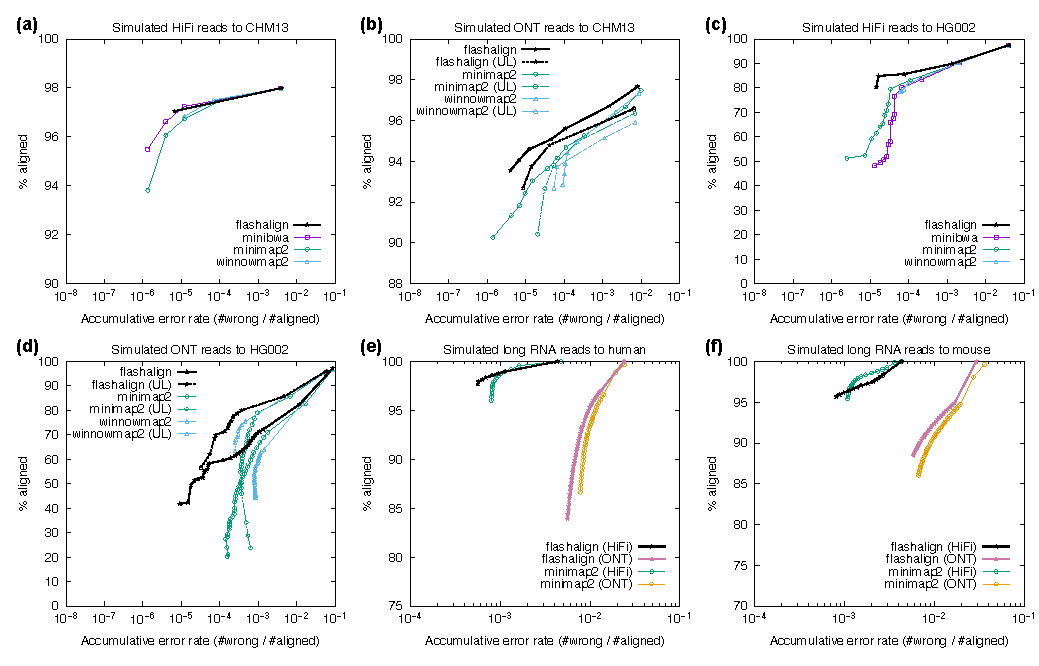
\includegraphics[width=0.95\textwidth]{figures/fig2_mapq.pdf}
\caption{Mapping accuracy on simulated long reads. Reads are simulated from T2T-CHM13, the diploid HG002 genome or LRGASP transcript models and mapped back to the source reference. Suppose a read originates from interval $G_s$ and is mapped to $G_a$. A read is considered as mapped correctly if $|G_s\cap G_a|/|G_s\cup G_a| \ge 10\%$. \textbf{(a,b)} HiFi and ONT reads simulated from T2T-CHM13. \textbf{(c,d)} HiFi and ONT reads simulated from the diploid HG002 genome. \textbf{(e,f)} LRGASP long RNA reads, human and mouse. Each ONT panel also carries that genome's ONT ultra-long cohort, as a second dashed arm of the same colour, labelled (UL).}
\label{fig:mapeval}
\end{figure*}

\begin{figure*}[t]
\centering
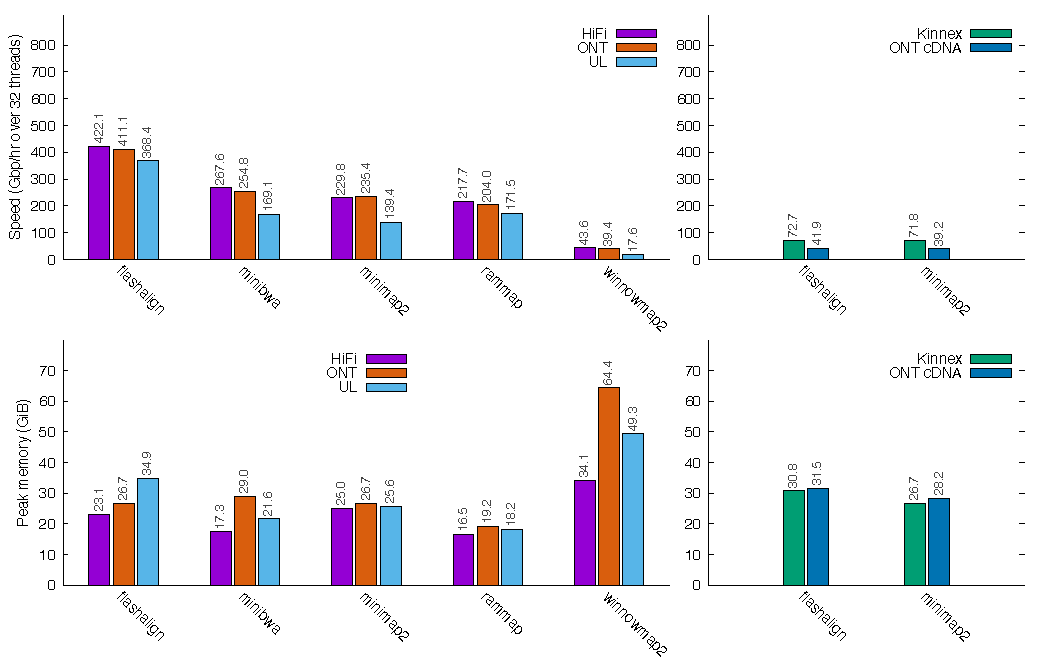
\includegraphics[width=0.95\textwidth]{figures/fig3_perf.pdf}
\caption{Speed and peak memory on real data. All tools in the panel are pinned to 32 threads, although Winnowmap2 consumed all 64 threads. PacBio HiFi and ONT are mapped to GRCh38 and ultra-long is mapped to T2T-CHM13v2.0. The RNA lanes are mapped to GRCh38 with GENCODE~44. All outputs of the aligners are sent to /dev/null.}
\label{fig:perf}
\end{figure*}


\section{Results}


We evaluated the mapping accuracy on simulated reads and measured the throughput performance on real data. We tested \flash{} v0.4.0, \mmtwo{} v2.31-r1302 \citep{li2018minimap2}, minibwa v0.7 \citep{li2026minibwa} and Winnowmap2 v2.03 \citep{jain2020winnowmap,jain2022winnowmap2}, with each tool's recommended preset over HiFi and ONT long reads. Minibwa over ONT long reads mapping accuracy evaluation is not shown, since their GitHub suggested it does not work for long noisy reads \citep{minibwa2026github}. All tools were run on a Linux workstation with an AMD Ryzen Threadripper 9970X 64-thread CPU at 5.0\,GHz.

\subsection{Mapping accuracy on simulated long reads}
\label{sec:res-dna}


We used the Badread \citep{wick2019badread} for simulated long reads. For PacBio HiFi reads, we use the \texttt{pacbio2021} models and for ONT used the \texttt{nanopore2023} models. All interior knobs match how minibwa \citep{li2026minibwa} reported recipe for simulation long reads dataset. Evaluation is calculated by mapping errors compared to the simulated position to the mapping position.

Figure~\ref{fig:mapeval} reports mapping accuracy in the style of \citet{li2026minibwa} and \citet{li2018minimap2}. A mapper of higher accuracy yields a curve closer to the upper-left corner. \flash{} is more accurate than all other tools. This is plainly because most tools use the same inherent seed--chain--align recipe while \flash{} added one more stage that can be informative enough for creating an improvement over the existing MAPQ formula.



We used the LRGASP simulated reads \citep{pardopalacios2024lrgasp} for making the RNA panels (e,f). Because other existing RNA long reads aligners don't have a proper MAPQ emission over the 0--60 range, the only comparison tool over RNA long reads is \mmtwo{}. All four lanes, human and mouse and HiFi and ONT, from LRGASP are being examined. From Figure~\ref{fig:mapeval}e and f, as shown, generally, \flash{} maps more while keeping the same or lower error rate as \mmtwo{}.


\subsection{Mapping performance}
\label{sec:res-perf}

\newcommand{\pend}{\textcolor{orange!80!black}{\textbf{pending}}}
\begin{table}[b]
\caption{Long-read structural variant calling on HG002 against the GIAB v5.0q truth. R recall, P precision.}
\label{tab:sv}
\footnotesize
\setlength{\tabcolsep}{2pt}
\begin{tabular*}{\columnwidth}{@{\extracolsep{\fill}}lrrrrrr@{}}
\toprule
 & \multicolumn{3}{c}{HiFi 37$\times$} & \multicolumn{3}{c}{ONT 60$\times$}\\
\cmidrule(lr){2-4}\cmidrule(lr){5-7}
 & R & P & F1 & R & P & F1\\
\midrule
\flash{} & \textbf{0.797} & 0.938 & \textbf{0.862} & \textbf{0.756} & 0.931 & \textbf{0.835}\\
\mmtwo{} & 0.785 & \textbf{0.944} & 0.857 & 0.749 & \textbf{0.941} & 0.834\\
minibwa & 0.776 & 0.916 & 0.841 & 0.740 & 0.925 & 0.822\\
Winnowmap2 & 0.745 & 0.924 & 0.825 & 0.730 & 0.933 & 0.819\\
\bottomrule
\end{tabular*}
\end{table}

\begin{table}[t]
\caption{Evaluation of junction accuracy on simulated ONT direct RNA reads}
\label{tab:rna}
\footnotesize
\begin{tabular*}{\columnwidth}{@{\extracolsep{\fill}}lrr@{}}
\toprule
 & \flash{} & \mmtwo{}\\
\midrule
\# aligned reads & 19\,969\,270 & 19\,783\,800\\
\# chimeric alignments & 7\,030 & 6\,635\\
\# non-spliced alignments & 4\,216\,935 & 4\,242\,046\\
\# aligned introns & 79\,892\,314 & 79\,290\,562\\
\# novel introns & 11\,464 & 26\,079\\
\% exact introns & 96.2 & 96.1\\
\% approx.\ introns & 99.1 & 99.1\\
\bottomrule
\end{tabular*}
\par\smallskip
{\scriptsize\noindent Notes: The 20 million LRGASP simulated mouse ONT direct RNA reads \citep{pardopalacios2024lrgasp} were mapped to the mouse genome GRCm39 with SIRV spike-ins with the following tools and command options: \flash{} (`\texttt{-{}-preset splice -u f}', index `\texttt{-k14}') and \mmtwo{} (`\texttt{-x splice -uf -k14}'). No gene annotation was given to either tool. The alignments were compared to the annotation the reads were simulated from: GENCODE M27 basic plus the human GENCODE 38 transcripts that LRGASP placed as novel isoforms. A predicted intron is novel if it has no overlaps with any annotated introns. An intron is exact if it is identical to an annotated intron. An intron is approximate if both its 5$'$- and 3$'$-end are within 10\,bp around the ends of an annotated intron. Chimeric alignments are supplementary alignments as defined in the SAM spec.\par}
\end{table}

We used several open source real reads dataset to evaluate our throughput performance on long reads compared to other aligners. For long genomic reads, we used the HG002 PacBio HiFi reads (\url{https://bit.ly/hg002-hprc-revio}), the HG002 Nanopore R10 reads (\nolinkurl{s3://ont-open-data/giab_2023}) and the HG002 Nanopore R10.4.1 ultra-long reads (HPRC bucket \nolinkurl{s3://human-pangenomics}, submission \texttt{UCSC\_GIAB\_R1041\_nanopore}, \texttt{HG002\_R1041\_UL}). For spliced long reads, we used the H69 cell line reads of the LongBench dataset \citep{you2025longbench} (\nolinkurl{s3://longbench-data/raw/fastq/}): PacBio Kinnex and ONT PCR-cDNA to GRCh38 with GENCODE~44.

\flash{} is the fastest tool for handling long genomic reads (Figure~\ref{fig:perf}). It is 1.7 to 2.6 times as fast as \mmtwo{} and the fastest tool on all three tested long-read datasets. The voting mechanism allows chaining to become much more versatile. On long spliced RNA reads, \flash{} is equal to or faster than \mmtwo{}. This is because the voting mechanism allows \flash{} to align spliced reads of longer length faster than \mmtwo{}. The longer the reads in the dataset, the faster \flash{} behaves on the spliced RNA dataset.


\subsection{Structural variant calling}
\label{sec:res-sv}


We aligned public long reads of HG002 from two platforms, PacBio Revio HiFi at $\sim$37$\times$ and ONT R10.4.1 SUP at 60$\times$, to T2T-CHM13v2.0 \citep{nurk2022chm13} with \flash{}, \mmtwo{} 2.31 \citep{li2018minimap2}, minibwa 0.7 \citep{li2026minibwa} and Winnowmap2 2.03 \citep{jain2022winnowmap2} at each tool's recommended long-read preset. As evaluated, \flash{} reaches the same or more biologically meaningful SV events compared to \mmtwo{} and other aligners at its more versatile throughput. We believe the exact form of chaining helps the performance of chaining become more accurate over long reads.

SVs were then called with Sniffles2 2.8.0 \citep{smolka2024sniffles2} at defaults and cuteSV 2.1.4 \citep{jiang2020cutesv} with \texttt{\mbox{-{}-genotype}}. Then they are compared to the GIAB v5.0q draft benchmark \citep{zook2020giab,giab2025v50q} with Truvari 5.4.0 \citep{english2022truvari} using the benchmark's recommended settings (\texttt{\mbox{-{}-pick}~ac \mbox{-{}-passonly} \mbox{-r~2000} \mbox{-C~5000}}) with refine mode on \citep{english2024tandem}. Table~\ref{tab:sv} gives the Sniffles2 numbers; cuteSV preserves the ordering. \flash{} achieves better recall in finding structural variant events while losing a little precision compared to \mmtwo{}. Overall, \flash{} is not only faster than \mmtwo{} and other tools but ready for downstream analysis such as variant calling.


\subsection{Spliced long reads}
\label{sec:res-rna}

We evaluated our performance on spliced long reads against \mmtwo{} on all four panels of spliced long reads from LRGASP. Overall, \flash{} maps more reads than \mmtwo{} (Table~\ref{tab:rna}), because the vote finds a plausible locus before chaining. Its MAPQ is also better calibrated: at the same threshold it places more reads with a lower error rate. The exception is the human ONT cDNA panel, where \flash{} is more conservative at Q60, keeping fewer reads with fewer errors.




\section{Discussion}

We developed \flash{} for aligning genomic long reads and spliced long reads to accelerate science that involves long sequencing data. It creates a breakthrough of the existing idea of diagonal compression before chaining that existed in aligners back to the GraphMap \citep{sovic2016graphmap} and minimap \citep{li2016minimap} time. On genomic long reads \flash{} is versatile enough to claim its novelty, and on spliced long reads \flash{} achieves better mapping accuracy without hurting throughput. We found the same algorithm can also be applied to contig mapping. We plan to work on that to ship the feature in the \flash{} package.

\section*{Acknowledgements}
We are thankful to Heng Li for writing such a magical ksw2 base-level alignment kernel on top of the Suzuki--Kasahara formulation \citep{suzuki2018difference}, and for his aligners minimap, \mmtwo{} and minibwa \citep{li2016minimap,li2018minimap2,li2026minibwa}, which gave us insights for making algorithm improvements.

\section*{Data availability}
{\footnotesize\raggedright\setlength{\parskip}{0pt}\setlength{\parindent}{0pt}\everypar{\hangindent=1em\hangafter=1}%
\flash{} source code: \url{https://github.com/97YearsOldProgrammer/flashalign}\par
HG002 PacBio HiFi reads: \url{https://bit.ly/hg002-hprc-revio}\par
HG002 Nanopore R10 reads: \url{s3://ont-open-data/giab_2023.05/}\par
HG002 Nanopore ultra-long reads: \url{s3://human-pangenomics/submissions/5b73fa0e-658a-4248-b2b8-cd16155bc157--UCSC_GIAB_R1041_nanopore/HG002_R1041_UL/}\par
LongBench H69 reads: \url{s3://longbench-data/raw/fastq/}\par
LRGASP simulated RNA reads: \url{https://cgl.gi.ucsc.edu/data/LRGASP/data/simulation/}\par}

\section*{Conflict of interest}
None declared.


\clearpage
\RefPageStart
\begingroup
\small
\setlength{\bibsep}{2.2pt plus 0.5pt}
\bibliography{refs}
\endgroup
\RefPageCheck
\end{document}
